% questions.tex —— 1977 年·黑龙江初试卷 · 题目内容片段（无答案）
% 由 tools/generate_projects.py 依来源总账自 1977/1977_数学真题_黑龙江初试_试题.md 生成，勿手改（改源 MD 后重跑）


\gkpart{数学试卷（黑龙江初试卷）}

\begin{gktip}
\textbf{来源说明}：本题面依据固定源 PDF《黑龙江省（初试）》第 1—3 页（原书页码 93—95）逐题转录。源材料为黑龙江省 1977 年高校招生初试（预选）数学试卷；与本库天津、河南等卷不同，源 PDF 每道题的题干下方直接连排印有推导过程与最终结果，并非纯题面卷。本文按流水线规范拆分为「试题」「答案要点」「解析正文」三份：答案要点与解析正文均由本库依据题面独立重新推导并对照源印解答复核，不逐字抄录源解答文字。原卷"考生须知"注明：①中专和技工学校考生回答第 1—9 题，高等学校考生回答第 4—12 题；②试卷只写题号，不抄题目；③答卷时间为 120 分钟。本文按 PDF 题序全部转录，共 12 题，原卷无附加题或参考题。
\end{gktip}

\par\medskip

\begin{question}
\gkti{1}\textbf{（10 分）} 计算：

\nopagebreak[4]
\[
\frac23-\frac12+0.3\times1.4\div0.6.
\]

\end{question}
\begin{question}
\gkti{2}\textbf{（10 分）} 计算：

\nopagebreak[4]
\[
-\frac13+2\times\left(-\frac23\right)^2-3^2\div\left(-1\frac12\right).
\]

\end{question}
\begin{question}
\gkti{3}\textbf{（10 分）} 已知圆的周长为 $12\pi\ \mathrm{cm}$，求这个圆的面积（$\pi=3.14$）。

\end{question}
\begin{question}
\gkti{4}\textbf{（10 分）} 解方程：

\nopagebreak[4]
\[
\frac{7}{2x+6}-\frac34=\frac{5}{x+3}.
\]

\end{question}
\begin{question}
\gkti{5}\textbf{（10 分）} 因式分解：

\nopagebreak[4]
\[
3a^2+6ab+3b^2-12c^2.
\]

\end{question}
\begin{question}
\gkti{6}\textbf{（10 分）} 试讨论 $a$ 与 $-a$ 的大小。

\Needspace{0.4\textheight}
\end{question}
\begin{question}
\gkti{7}\textbf{（15 分）} 已知 $AB\text{、}AC$ 是 $\odot O$ 的切线，$B\text{、}C$ 是切点，$\angle BAC=120^\circ$，$AO=10\ \mathrm{cm}$，求 $\odot O$ 的半径和切线 $AB$ 的长。
\nopagebreak[4]
\begin{center}% 1977 年黑龙江初试卷第 7 题：⊙O 的两条切线 AB、AC，切点 B、C，∠BAC=120°（按源卷第 2 页布局）
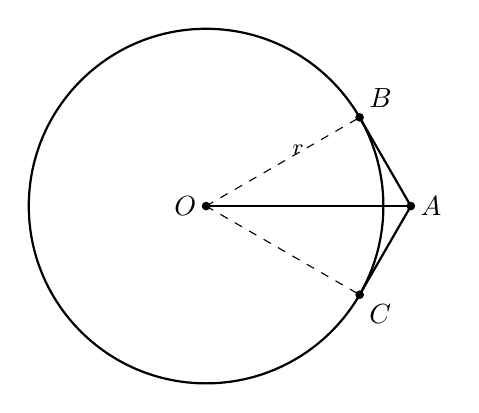
\begin{tikzpicture}[scale=1.3]
  \coordinate (O) at (0,0);
  \coordinate (A) at (2,0);
  \coordinate (B) at (1.5,0.866);
  \coordinate (C) at (1.5,-0.866);
  \draw[thick] (O) circle (1.732);
  \draw[thick] (A)--(B);
  \draw[thick] (A)--(C);
  \draw[thick] (O)--(A);
  \draw[dashed] (O)--(B);
  \draw[dashed] (O)--(C);
  \fill (O) circle (1.2pt) node[left] {$O$};
  \fill (A) circle (1.2pt) node[right] {$A$};
  \fill (B) circle (1.2pt) node[above right] {$B$};
  \fill (C) circle (1.2pt) node[below right] {$C$};
  \node at (0.9,0.55) {\footnotesize $r$};
\end{tikzpicture}
\end{center}
\nopagebreak[4]
\Needspace{0.4\textheight}
\end{question}
\begin{question}
\gkti{8}\textbf{（10 分）} 在直角 $\triangle ABC$ 中，$\angle C=90^\circ$，$CD\perp AB$。求证：

\nopagebreak[4]
\[
\frac{CD}{AD}=\frac{BD}{CD}.
\]
\nopagebreak[4]
\begin{center}% 1977 年黑龙江初试卷第 8 题：直角三角形 ABC，∠C=90°，CD⊥AB，D 为垂足，∠1=∠BCD，∠2=∠ACD（按源卷第 2 页布局）
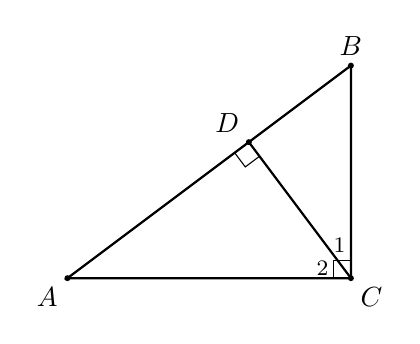
\begin{tikzpicture}[scale=0.9]
  \coordinate (A) at (0,0);
  \coordinate (C) at (4,0);
  \coordinate (B) at (4,3);
  \coordinate (D) at (2.56,1.92);
  \draw[thick] (A)--(B)--(C)--cycle;
  \draw[thick] (C)--(D);
  \draw (3.75,0)--(3.75,0.25)--(4,0.25);
  \draw (2.36,1.77)--(2.51,1.57)--(2.71,1.72);
  \fill (A) circle (1.2pt) node[below left] {$A$};
  \fill (B) circle (1.2pt) node[above] {$B$};
  \fill (C) circle (1.2pt) node[below right] {$C$};
  \fill (D) circle (1.2pt) node[above left] {$D$};
  \node at (3.84,0.47) {\footnotesize $1$};
  \node at (3.6,0.14) {\footnotesize $2$};
\end{tikzpicture}
\end{center}
\nopagebreak[4]
\end{question}
\begin{question}
\gkti{9}\textbf{（15 分）} 甲、乙两个车间按计划每月共生产 $450$ 件产品，粉碎“四人帮”之后，在工业学大庆运动的推动下，甲车间完成了计划的 $120\%$，乙车间完成了计划的 $110\%$，两车间共生产 $515$ 件产品，问甲、乙两车间原计划各生产多少件产品？

\end{question}
\begin{question}
\gkti{10}\textbf{（10 分）} 计算（不查表）：

① $\sin(-510^\circ)$；

② $\left(\dfrac12\right)^{-2}-9^{\frac12}+5^0-\sqrt2\cdot\sqrt8+\log_77$。

\Needspace{0.4\textheight}
\end{question}
\begin{question}
\gkti{11}\textbf{（10 分）} 在 $\triangle ABC$ 中，已知 $\angle A=120^\circ$，$\angle B=45^\circ$，$AC=6\ \mathrm{cm}$，求 $BC$ 的长。
\nopagebreak[4]
\begin{center}% 1977 年黑龙江初试卷第 11 题：△ABC 中 ∠A=120°，∠B=45°，AC=6cm（按源卷第 3 页布局）
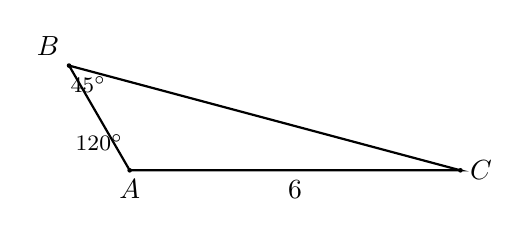
\begin{tikzpicture}[scale=0.7]
  \coordinate (A) at (0,0);
  \coordinate (C) at (6,0);
  \coordinate (B) at (-1.1,1.9);
  \draw[thick] (A)--(B)--(C)--cycle;
  \fill (A) circle (1.2pt) node[below] {$A$};
  \fill (B) circle (1.2pt) node[above left] {$B$};
  \fill (C) circle (1.2pt) node[right] {$C$};
  \node at (-0.55,0.5) {\footnotesize $120^\circ$};
  \node at (-0.75,1.55) {\footnotesize $45^\circ$};
  \node at (3,-0.35) {$6$};
\end{tikzpicture}
\end{center}
\nopagebreak[4]
\end{question}
\begin{question}
\gkti{12}\textbf{（10 分）} 求函数 $y=-x^2-2x+3$ 的最大值。

\end{question}